\documentclass{../custom_packages} % deficao da classe e das opcoes do documento
\begin{document}
	
%%% *******************************
%%% Capa
%%% *******************************
\begin{titlepage}
\begin{center}
\textbf{\Large Laboratoire TIMA}\\[0.3cm] 
\textbf{\large Équipe AMfoRS}\\[0.1cm]
%\textbf{\large Engenharia Elétrica}\\[0.1cm]
\vspace{20pt}

\includegraphics[scale=0.4]{../images/capa-tima.png}\\[1cm]

\par
\vspace{20pt}
\textbf{\LARGE Projet SysAx}\\
\vspace{15pt}
\textbf{--------------------------------------------------------------------------------}\\
\textbf{\large Self-adaptative approximate SoC: HW platform development}\\
\vspace{15pt}
\textbf{\Large Bref regarde sur la platforme PULP}\\
\textbf{--------------------------------------------------------------------------------}\\
%\myrule[1pt][7pt]
\vspace{35pt}
%\textbf{\large Aluno \hspace{60pt} Matrícula}\\
\textbf{\large Auteur :}\\[0.1cm]
Gabriel Villanova N. Magalhães\\
%111150346
%Gabriel Villanova \hspace{50pt} 111150346 \\

\vspace{45pt}
\textbf {\large Conseiller :}\\[0.2cm]
\Large {Dr. Mounir BENABDENBI}\\[0.1cm]
\end{center}

\par
\vfill
\begin{center}
\textbf{Date : mars / 2018	}\\
\end{center}

\end{titlepage}

%%% *******************************
%%% Sumário 
%%% *******************************
\cftsetindents{section}{0em}{2em}
\cftsetindents{subsection}{0em}{2em}


\renewcommand\lfttoctitlefont{\hfill\Large\bfseries}
\renewcommand\lftaftertoctitle{\hfill\mbox{}}

\tableofcontents
\thispagestyle{empty}
\newpage
\thispagestyle{empty}
%%% *******************************
%%% Lista de Figuras e Tabelas
%%% *******************************
\listoffigures
\thispagestyle{empty}
\newpage

%\pagestyle{fancy}
%\setcounter{page}{1}
%\thispagestyle{empty}
%\listoftable
%\thispagestyle{empty}
%\newpage

\addtocontents{toc}{\protect\thispagestyle{empty}}
\pagestyle{fancy}
\setcounter{page}{1}

%%% *******************************
%%% Capitulos
%%% *******************************
\section{PULP}

\subsection{Bref étude sur plataform PULP et caractéristique des hws}

Dans ce section on va présenter l'objectif et recherche du projet PULP développé pour le labo ETH Zurich et Université de Bologna. En plus, on montre le type de hardware et le framework qu'ils offrent actuellement pour utiliser le projet.

Des objectifs et recherche, on souligne :

\begin{itemize}[noitemsep]
	\item arriver à 1GOPS/mW d'efficacité ;
	\item \textbf{scalabilité hw en efficacité d'energie} :
		\subitem plus hw or modif. hw pour plus d'efficacité d'energie.
	\item exploit le parallelism :
		\subitem multiple petit-cores dans un cluster ;
		\subitem partage de memoire avec le cluster.
	\item \textbf{cores simplifiés, mais efficace} ;
	\item optimization du hw ;
	\item accelerateurs dediés ;
	\item \textbf{extension d'isa pour des nécessités sw} :
		\subitem ajout de instructions (e.g. hw loops).
	\item projet \textit{open-source}.
\end{itemize}

À partir de toutes ces idées et objectifs, un ensemble de travaux ont été développé et testés. En exploitant le repository du projet (\url{https://github.com/pulp-platform/pulp}), on peut voir que c'est un framework simples (essentiellement avec des ips et test benches), mais qui contient beaucoup de possibilités pour construire des hardwares différentes. La figure \ref{fig:ips} montre toutes les ips disponibles.

\begin{figure}[H]
 \centering
 \begin{small}
    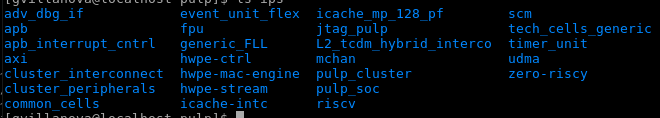
\includegraphics[scale=.7]{../images/ips-pulp.png}
 \end{small}
  \caption{IPs disponibles dans plataform PULP.}
  \label{fig:ips}
\end{figure}

On peut voir que les ips des \textbf{cores} (riscv et zero-riscy) sont séparés, ainsi que les parties pour construir les SoCs, ça inclut : bus, memoires du type cache, périphériques, top-level niveau cluster, top-level niveau SoC, etc. Ça donne plusieurs possibilités de travailler dans ce repositoire. 

Comme par exemple : 

\begin{itemize}[noitemsep]
	\item exploiter \textbf{le single-core riscv };
	\item exploiter \textbf{le single-core zero-riscy };
	\item exploiter \textbf{le SoC avec riscv (8 cores in cluster, projet PULP)} ;
	\item exploiter \textbf{le SoC avec zero-riscy (8 cores incluster,projet PULP)}.
\end{itemize}

Pour comprendre la complexité des ces hardwares, on liste les caractéristiques des cores  :

\begin{itemize}[noitemsep]
	\item \textbf{riscv or riscy} :
 		\subitem \textbf{architeture 32 bits} ;
 		\subitem 4 niveau de pipeline ;
 		\subitem implementation d'ISA RVICMF.

\begin{figure}[H]
 \centering
 \begin{small}
    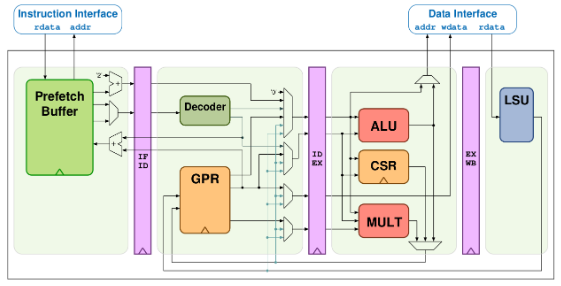
\includegraphics[scale=.7]{../images/riscy-arc.png}
 \end{small}
  \caption{Architeture générale RISCY.}
  \label{fig:riscy-arc}
\end{figure}

	\item \textbf{zero-riscy} :
 		\subitem \textbf{architeture 32 bits} ;
 		\subitem 2 niveau de pipeline ;
 		\subitem implementation d'ISA RVICME.
\end{itemize}

Le riscy et zero-riscy sont \textbf{cores stables} et ils ont une \textbf{toolchain espécifique} (aussi stable) pour création de \textbf{software}  pour eux. La figura \ref{fig:pulp-arc} (architeture aussi de 32 bits), montre le SoC qu'utilise ces cores, il utilise \textbf{8 cores} en travaillant ensemble dans un cluster, ça montre à-peu-près le niveau complexité du parallelism que le PULP forni. Enfin, \textbf{le SoC est stable} et \textbf{il n'y a pas de support pour le linux embarqué} (or similaire), par contre \textbf{supporte RTOS} (e.g. freeRTOS) pour être un \textbf{SoC du type microntroller}. 

\begin{figure}[H]
 \centering
 \begin{small}
    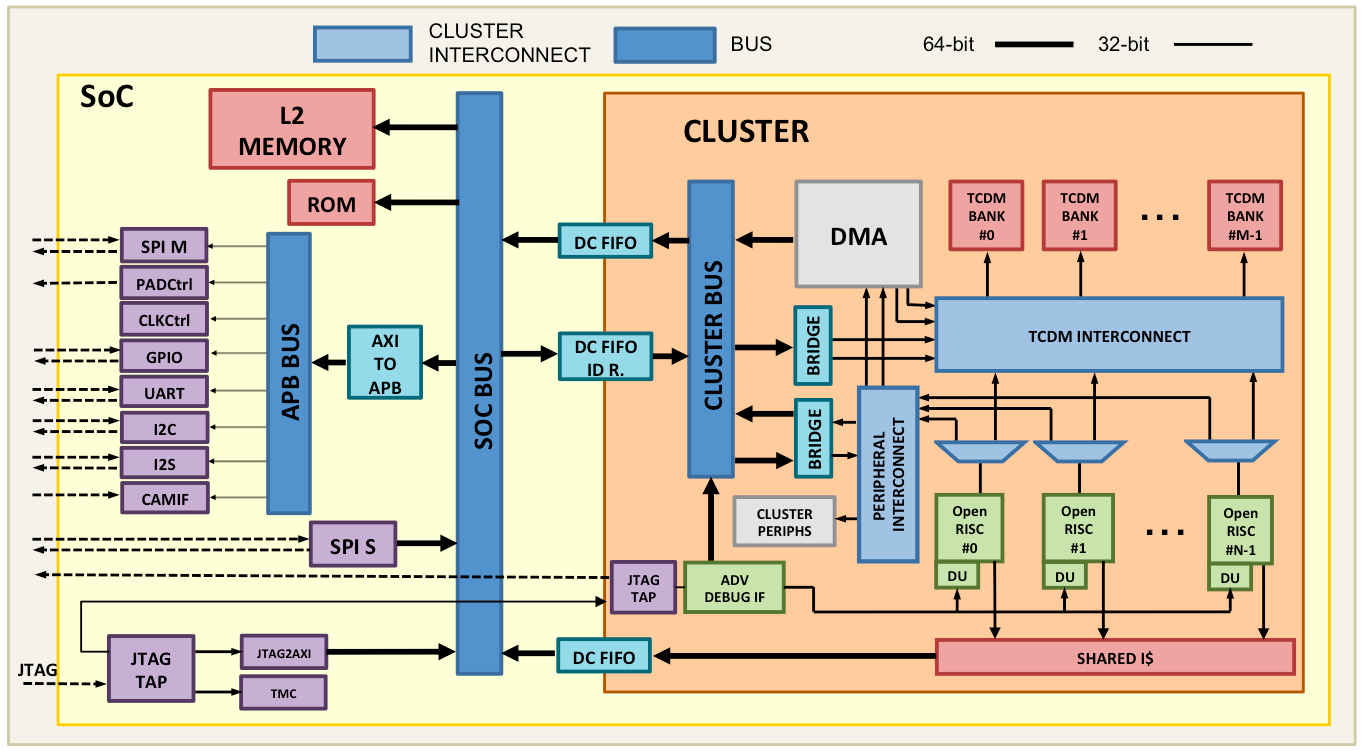
\includegraphics[scale=.33]{../images/pulp-arc.png}
 \end{small}
  \caption{Architeture générale du SoC PULP.}
  \label{fig:pulp-arc}
\end{figure}

Il y a encore autres outils pour exploiter, e.g. \textbf{le pulp-sdk (\textit{Software Development Kit})} qui peut forni plus de possibilités pour exploiter cette platform. 

\newpage
\subsection{Quelquels résultats}

Ce section présenterai quelques \textbf{tests basiques avec le ip core riscv}, ça montrerait comme c'est \textbf{facile d'utiliser ce système et le porter pour l'utiliser dans un nouvelle projet}, comme par example, le projet SysAx. Une fois le core bien piloté pour nous et avec la compréhension de l'utilisation du SoC PULP, on peut avancer sur le sujet \textit{\textbf{Approximate Computing}} autant que dans le single core comme dans le SoC complet, en permettant plusieurs types d'usage.

Dans ces tests on a utilisé les suivants softwares, sur le OS Fedora 24 : 

\begin{itemize}[noitemsep]
	\item ModelSim Student Version 10.5b ;
	\item Vivado 2016.4 ;
	\item Verilator 3.890.
\end{itemize}

Pour des tests avec le ModelSim, une propre structure a été fait, en portent les sources su directoire /pulp/ips/riscv et en créant notre propre repository. La figure \ref{fig:dir-ms} montre l'organisation fait.
\\
\begin{figure}[H]
 \centering
 \begin{small}
    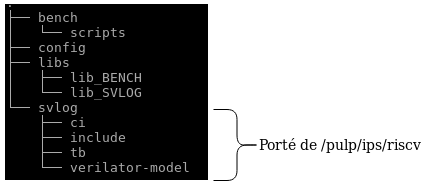
\includegraphics[scale=.85]{../images/dir-ms-full.png}
 \end{small}
  \caption{Structure de simulation core riscy.}
  \label{fig:dir-ms}
\end{figure}

À partir de ça, on a fait un simples script pour compiler les sources du (*.sv) du ip core, en utilisant le ModelSim. On peut voir les sources et les commandes utilisés dans le code suivant : 

\newpage 
\begin{lstlisting}[language=bash,caption={compil\_SVLOG.sh}]
vdel -lib  ${PATH_WORK}/libs/lib_SVLOG -all

vlib ${PATH_WORK}/libs/lib_SVLOG

vmap lib_SVLOG ${PATH_WORK}/libs/lib_SVLOG 

vlog +incdir+./include -work lib_SVLOG ./include/apu_core_package.sv
vlog +incdir+./include -work lib_SVLOG ./include/apu_macros.sv
vlog +incdir+./include -work lib_SVLOG ./include/riscv_config.sv
vlog +incdir+./include -work lib_SVLOG ./include/riscv_defines.sv
vlog +incdir+./include -work lib_SVLOG ./include/riscv_tracer_defines.sv

vlog +incdir+./include -work lib_SVLOG riscv_L0_buffer.sv
vlog +incdir+./include -work lib_SVLOG riscv_fetch_fifo.sv
vlog +incdir+./include -work lib_SVLOG riscv_apu_disp.sv
vlog +incdir+./include -work lib_SVLOG riscv_alu.sv 
vlog +incdir+./include -work lib_SVLOG riscv_alu_basic.sv
vlog +incdir+./include -work lib_SVLOG riscv_alu_div.sv
vlog +incdir+./include -work lib_SVLOG riscv_compressed_decoder.sv
vlog +incdir+./include -work lib_SVLOG riscv_controller.sv
vlog +incdir+./include -work lib_SVLOG riscv_cs_registers.sv
vlog +incdir+./include -work lib_SVLOG riscv_debug_unit.sv
vlog +incdir+./include -work lib_SVLOG riscv_decoder.sv
vlog +incdir+./include -work lib_SVLOG riscv_int_controller.sv
vlog +incdir+./include -work lib_SVLOG riscv_ex_stage.sv
vlog +incdir+./include -work lib_SVLOG riscv_hwloop_controller.sv
vlog +incdir+./include -work lib_SVLOG riscv_hwloop_regs.sv
vlog +incdir+./include -work lib_SVLOG riscv_id_stage.sv
vlog +incdir+./include -work lib_SVLOG riscv_if_stage.sv
vlog +incdir+./include -work lib_SVLOG riscv_load_store_unit.sv
vlog +incdir+./include -work lib_SVLOG riscv_mult.sv
vlog +incdir+./include -work lib_SVLOG riscv_prefetch_buffer.sv
vlog +incdir+./include -work lib_SVLOG riscv_prefetch_L0_buffer.sv
vlog +incdir+./include -work lib_SVLOG riscv_core.sv
\end{lstlisting}

Le résultat de compilation n'a pas reporté des erreurs. Pour utiliser le core, on a porté le test-bench tb.sv forni, en compilant comme ça :
\\
\begin{lstlisting}[language=bash,caption={compil\_BENCH.sh}]
vdel -lib  ${PATH_WORK}/libs/lib_BENCH -all
vlib ${PATH_WORK}/libs/lib_BENCH
vmap lib_BENCH ${PATH_WORK}/libs/lib_BENCH

vlog -work lib_SVLOG tb.sv
\end{lstlisting}

Les codes du ip riscv, ainsi que du tb.sv sont recontré dans le repository pulp originale. Ce tb.sv utilise seulment l'unité riscv\_alu\_div.sv, comme ça, c'est une espèce de kick-off que la plataform nous donne pour exploiter et écrit des testes pour les autres unité et le core complet. Quelques formes d'onde de l'application sont montré dans la figure \ref{fig:wave-alu}, en montrant le succès du test.

\begin{figure}[H]
 \centering
 \begin{small}
    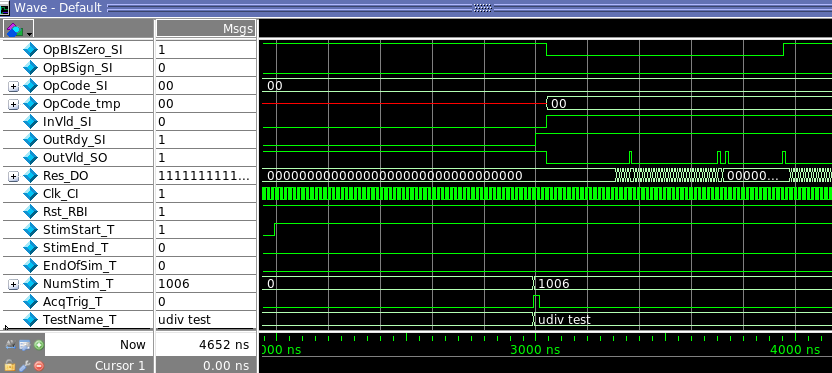
\includegraphics[scale=.55]{../images/wave-alu.png}
 \end{small}
  \caption{Waves formes d'unité riscv\_alu\_div.sv.}
  \label{fig:wave-alu}
\end{figure}

Dans le dossier \textbf{verilator-model} est forni un test-bench pour le ip-core complèt écrit avec C++. En faisant juste un  <<$ $ \$ make $ $>> sur ce dossier et on a des sorties de compilation imprimé sur le terminal ainsi que les waves formes. 

\begin{figure}[H]
 \centering
 \begin{small}
    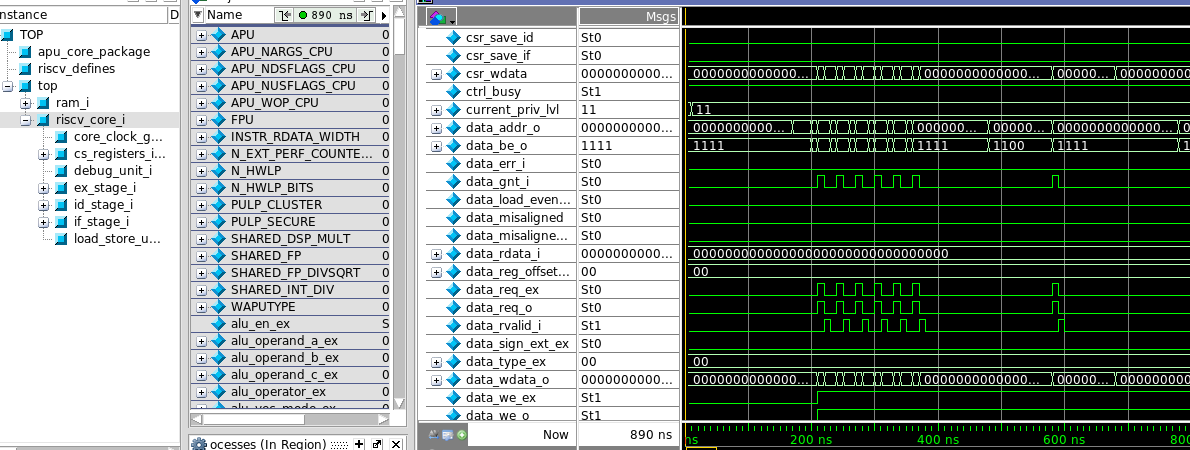
\includegraphics[scale=.38]{../images/wave-riscv.png}
 \end{small}
  \caption{Waves formes du processeur riscy.}
  \label{fig:wave-alu}
\end{figure}

Le <<$ $ load$ $ >> du program dans la memoire d'instruction est fait dans le code du test-bench.cpp. Donc, on peut le modifier pour vérifier autres functionalités du processeur.

Comme ça, on voit que le principale core de la platform pulp marche dans le niveau de simulation. Alors, on a aussi essayé de faire la synthèse, niveau RTL sur Vivado, et avec un peu de modification dans les codes, c'est possible de le synthetiser comme on peut voir dans la figure \ref{fig:viv-riscv}.  

\begin{figure}[H]
 \centering
 \begin{small}
    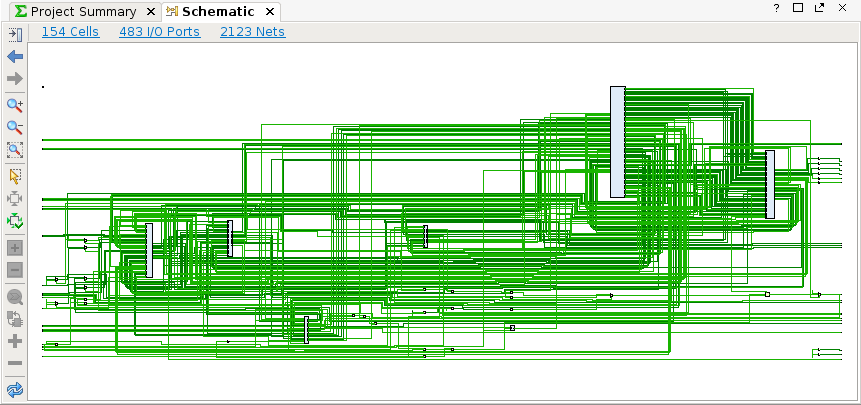
\includegraphics[scale=.5]{../images/viv-riscv.png}
 \end{small}
  \caption{Synthèsis niveau RTL du riscy sur Vivado.}
  \label{fig:viv-riscv}
\end{figure}

\subsubsection{Les possibilités des nouvelles tests}
\begin{itemize}[noitemsep]
	\item Créer des sw avec la PULP-toolchain pour les cores et les re-simuler ;
	\item Simuler le SoC (cluster + interfaces) ;
	\item Créer des sw pour le SoC ;
	\item Synthetiser le SoC dans FPGA.
\end{itemize}
\newpage
\subsection{Résume des avantages et désavantages}

\noindent
\textbf{Avantages} : 
\begin{itemize}[noitemsep]
\item le projet PULP cherche efficacité d'energie ;
\item les cores sont simples (32 bits, 4 or 2 niveau de pipeline), mais efficaces ;
\item ils ont fait extension d'ISA, cette méthodologie peut-être utiliser pour mettre extension de l'approximate computing ;
\item le sources du repositoire sont faciles de manipuler, comme ça c'est facile créer notre propres scripts dedans pour la simulation, tests et synthesis ;
\item il y a beaucoup des ips I/O : i2c, gpio, uart, etc.
\item il y a interface AMBA/APB dans le SoC, donc les projets chez PHELMA peuvent être fait avec ces interfaces pour qu'on puisse les utiliser à partir du SoC. 
\end{itemize}

\textbf{Desavantages} :
\begin{itemize}[noitemsep]
	\item Le hw que on peut créer sont limités, puisque les possibilités dans la plataform Rocket est énorme ;
	\item Il n'y a pas de support pour le linux embarqué (ou similaire), juste RTOS (e.g. freeRTOS) pour être un SoC du type Microntroller ;
	\item Le repositoire n'a pas gros contribuitions, juste le basique pour la simulations des ips ;
\end{itemize}

%%% ******************************
%%% Referências
%%% *******************************
\begin{thebibliography}{2}
\bibitem{ref1} \url{https://riscv.org/wp-content/uploads/2015/06/riscv-pulp-workshop-june2015.pdf}.
\bibitem{ref2} \url{http://iis-projects.ee.ethz.ch/index.php/PULP}.
\end{thebibliography}

\end{document}

%%%%%%%%%%%%%%%%%%%%%
%%% FIGURA %%%%%%%%%%
%%%%%%%%%%%%%%%%%%%%%
%\begin{figure}[H]
% \centering
% \begin{small}
%    \includegraphics[scale=.9]{grafico.jpg}
% \end{small}
%  \caption{Gráfico dos valores obtidos no experimento}
%  \label{fig:grafico}
%\end{figure}

%%%%%%%%%%%%%%%%%%%%%
%%% ITEMS %%%%%%%%%%%
%%%%%%%%%%%%%%%%%%%%%
%\begin{itemize}
%  \item Controle ON/OFF de postes de luz;
%  \item Sistema de segurança (alarme) para shoppings, bancos, etc...
%  \item Controle de intensidade de lâmpadas;
%  \item Medidores de luz;
%  \item Detectores de incêndio/fumaça;
%\end{itemize} 

%%%%%%%%%%%%%%%%%%%%%%%
%%% EQUACAO %%%%%%%%%%%
%%%%%%%%%%%%%%%%%%%%%%%
%\begin{eqnarray}
%TensaoX(\theta) = +1.5\sin(\theta)
%TensaoY(\theta) = -1.5\sin(\theta)
%\end{eqnarray}

%%%%%%%%%%%%%%%%%%%%%%%
%%% CODIGO %%%%%%%%%%%%
%%%%%%%%%%%%%%%%%%%%%%%
%\makeatletter
%\newenvironment{CenteredBox}{% 
%\begin{Sbox}}{% Save the content in a box
%\end{Sbox}\centerline{\parbox{\wd\@Sbox}{\TheSbox}}}% And output it centered
%\makeatother

%\begin{figure}[htb]
%\begin{CenteredBox}
%\begin{lstlisting}
% code here
%\end{lstlisting}
%\end{CenteredBox}
%\end{figure}

%%%%%%%%%%%%%%%%%%%%%%%
%%% TABELA %%%%%%%%%%%%
%%%%%%%%%%%%%%%%%%%%%%%
%\begin{table}[H] \footnotesize % Diminui tamanho de fonte na tabela
%\centering
%\begin{tabularx}{\textwidth}{| l | l | l |}
%hline
%\rowcolor[HTML]{EFEFEF}

%Pseudonome & Componente & Função \\ \hline
%Sensor de presença A & Sensor de obstáculo IR & Detectar usuário no nível superior \\ \hline
%Sensor de presença B & Sensor de obstáculo IR & Detectar usuário no nível inferior \\ \hline
%Motor para rotação & Motor de passo: ??? & Girar a parede de escalada \\ \hline
%Driver motor rotação & Driver: ??? & Cria interface de controle MCU-Motor \\ \hline
%Motor para inclinação & Motor de passo: ??? & Inclinar parede de escalada \\ \hline
%Driver motor inclinação & Driver: ??? & Cria interface de controle MCU-Motor \\ \hline
%Sensor de peso & Células de carga (50Kg) & Detectar usuário sobre piso \\ \hline
%MCU & Microcontrolador PIC16F877A & Controlar todos os componentes elétricos \\ \hline

%\end{tabularx}
%\caption{BOM: Bill of Material para projeto em miniatura}
%\label{tab:componentes_eletricos_mini}
%\end{table}

%%%%%%%%%%%%%%%%%%%%%%%%%%%
%%% REFERENCIA %%%%%%%%%%%%
%%%%%%%%%%%%%%%%%%%%%%%%%%%
%\begin{thebibliography}{2}
%\bibitem{ref1} Alberto Simões ,{\em Uma não tão pequena introdução ao \LaTeX},2007.
%\bibitem{ref2} Autor do livro ,{\em Título do Livro}, Ano de edição,Editora,etc.
%\end{thebibliography}

%%%%%%%%%%%%%%%%%%%%%%%%%%%%%%%%%%%%%%%%%
%%% Histórico de Revisões %%%%%%%%%%%%%%%
%%%%%%%%%%%%%%%%%%%%%%%%%%%%%%%%%%%%%%%%%
%\section{Histórico de Revisões}

%\begin{table}[h]
%\centering
%\begin{tabular}{|c|c|c|c|}
%\hline
%\rowcolor[HTML]{EFEFEF}

%Date & Version & Description & Author \\ \hline
%Data & Versão & Descrição & Autor \\ \hline
%01/03/2017 & 1.0 & Initial Release & Gabriel Villanova\\ \hline
%\end{tabular}
%\end{table}

% coloca em  branco o resto da página
%\hfill 
%\newpage